\documentclass{llncs}

% choose options for [] as required from the list
% in the Reference Guide, Sect. 2.2

\usepackage{makeidx}     % allows index generation
\usepackage{graphicx}    % standard LaTeX graphics tool
                         % when including figure files
\usepackage{amsmath,amsfonts,bbm} % used for the two-column index
\usepackage{color}%
\usepackage{longtable}
\usepackage{subfig}
\usepackage{cite}
\usepackage{nicefrac}
%\usepackage{refcheck}


% math definitions
\newcommand{\M}[1]{\mathbf{#1}}
\newcommand{\V}[1]{\mathbf{#1}}
\newcommand{\trace}[1]{\mbox{trace}\left( #1 \right)}
\newcommand{\VNull}{{\textbf{\em 0}}}
\newcommand{\norm}[1]{\left | \left | #1 \right | \right |}
\newcommand{\RR}{\mathbbm{R}}
\newcommand{\eps}{{\epsilon}}
\renewcommand{\epsilon}{\varepsilon}

\renewcommand\floatpagefraction{1}
\renewcommand\topfraction{1}
\renewcommand\bottomfraction{1}
\renewcommand\textfraction{0}

\newcommand{\gs}{Google SketchUp }

\title{Localizing Google SketchUp Models in Outdoor 3D Scans}

\titlerunning{Localizing Google SketchUp Models}

\author{Flavia Grosan, Alexandu Tandrau, and Andreas N{\"u}chter}

\authorrunning{F.Grosan, A.Tandrau, A.N{\"u}chter}


\institute{Jacobs University Bremen gGmbH\\
School of Engineering and Science, Automation Group\\
Campus Ring 12, 28759 Bremen, Germany\\
\email{\{f.grosan|a.tandrau|a.nuechter\}@jacobs-university.de}\\[2ex]
}

\begin{document}

\maketitle
  
%\frontmatter          % for the preliminaries

\pagestyle{headings} % switches on printing of running heads

\addtocmark{Title goes here again?} % additional mark in the TOC

\begin{abstract}
This work introduces a novel solution for localizing objects based on
search strings and freely available \gs models. To this end we
download and preprocess a collection of 3D models to obtain equivalent
point clouds. The outdoor scan is segmented into individual objects,
which are sequentially matched with the models by a variant of
iterative closest points algorithm using seven degrees of freedom and
resulting in a highly precise pose estimation of the object. An error
function evaluates the similarity level. The approach is verified
using various segmented cars and their corresponding 3D models.
\end{abstract}

\section{Introduction}

%\subsection{3D Laser Scanning and SLAM}

One fundamental topic in mobile robotics is simultaneous mapping and
localization (SLAM). In SLAM, the robot builds a map without prior
information about its positions. Laser range scanners are helpful in
solving SLAM since they provide a series of scans taken from different
poses.  To obtain a complete, consistent and precise map of the
exploration site, scans are often matched with iterative closest
points algorithm~\cite{Nuechter:2010}. This algorithm is commonly used in real
time and it iteratively alters the rigid-body transformations needed
to minimize the distance between consecutive scans. Finally a
GraphSLAM relaxation algorithm is used to refine the map and to yield
high precise pose estimates~\cite{Thrun:2005}.

Once the world is mapped, the next step towards a knowledge based
robotic system is obtaining semantic information about the environment
and thus enabling the robot to understand and interact efficiently
with the exploration site. A semantic map adds information to the
obtained scene by identifying static objects or dynamic
events. Through localization the robot determines where a particular
object is found.
%
Our approach towards semantic mapping takes advantage of the large
amount of information publicly available on the Internet. Google
Warehouse, a vast collection of user-made 3D models, offers valuable
content. For instance, given a precise goal ("There is a BMW Z3 in the
environment. Go find it!"), the robot downloads the 3D models
available for this object, converts them into 3D cloud points and the
localization process is then simplified to common scan matching with
an additional attention to scale (Fig.~\ref{model_scan}).

\begin{figure}
  \centering
    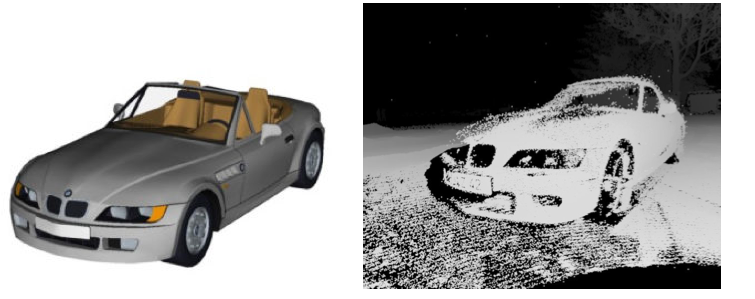
\includegraphics[width=0.5\textwidth]{model_scan}
  \caption{Left: 3D model BMW Z3 found in \gs Warehouse. Right: Actual car in a 3D laser scan.}
  \label{model_scan}
\end{figure}


\section{Related Work}

3D models are becoming the standard representation in applications
ranging from the medical sector to architecture. They are used for
visualization and object design because both humans and machines
interact with them naturally~\cite{Remondino:2009,Beetz:2010}.
%
Tangelder et al. discuss ways in which models are queried based on
text and shape~\cite{Tangelder:2004}. The similarity between objects
is achieved using the nearest neighbor algorithm and improves the scan
matching process. The scans are matched using iterative closest points
algorithm (ICP). Given an initial relative distance between two scans,
ICP matches points and computes an estimate of the transformation
between the two states. The process is repeated until
convergence. Horn proposed a closed form solution of absolute
orientation using unit quaternions, which supports all the basic
geometric transformations (translation, rotation and scale)
\cite{Horn:1987}.

N\"uchter et al. \cite{Nuchter:2008} make use of SLAM and ICP to
achieve semantic mapping. After determining the coarse scene features
(e.g, walls, floors), a trained classifier identifies more delicate
objects. Our work improves the semantic map by creating an even finer
differentiation between objects in the environment.

Object localization is another application of 3D models. The robot is
given a precise target to detect in an unknown environment. Kestler et
al. use a probabilistic representation. The targets are modeled in a
knowledge base (descriptive identifiers and attributes) and spatial
inference. Feature detection and hierarchical neural net
classification are used for object identification, while robot
localization is solved through sensor fusion, spatial abstraction and
multi-level spatial representations~\cite{Kestler:2000}. The drawback
of this approach is the need to maintain internal, neural net trained
data. Recently, Lai and Fox treat the aforementioned problem and
propose the use of Google Warehouse for training classifiers in order
to improve and extend object detection~\cite{Lai:2010}. The classifier
is based on a distance function for image features, which are obtained
via spin images implemented by Johnson and
Hebert~\cite{Hebert:1999}. The objects in the outdoor environment are
classified in seven categories: cars, people, trees, street signs, fences,
buildings and background. The paper does not give a solution for
identifying very precise targets, e.g., a BMW Z3. We solve this
problem, thus taking an extra step within the field of object
recognition and localization.

Hertzberg et al. use CAD models to introduce semantics in maps obtained with SLAM ~\cite{Hertzberg:2011}. They created an ontology modeling relationships between objects in an indoor environment scene and use standard ICP to match objects with their corresponding CAD models. The main disadvantage of this approach is the need to store size information in the ontology about the scan components, problem mitigated in this work through our implementation of ICP with scale.

\section{Obtaining Point Clouds from 3D Models}

Google 3D Warehouse is a collection of user made SketchUp
models. Thousands of models are freely available and searchable by
strings or tags. A SketchUp model is composed of different entities,
i.e., Face, ComponentInstance, or Group. A Face is a triangle defined
by three 3D points. ComponentInstances and Groups are entities (with
an associated transformation) recursively composed of other
entities. Any model is decomposed into a list of faces defined by
their respective points. The obtained point clouds are not uniformly
sampled, thus requiring an additional sampling procedure. Our sampling
procedure adds random points inside each triangular face
proportionally to the area of the triangle. We center the point clouds
in their respective centroid and bound the coordinates in $[-\alpha,
  \alpha]$ to avoid initial transformations which hinder the matching
algorithm in the following steps. Fig.~\ref{audia4resampled} shows
an Audi A4 model before and after the sampling procedure.

  \begin{figure}
    \centering
    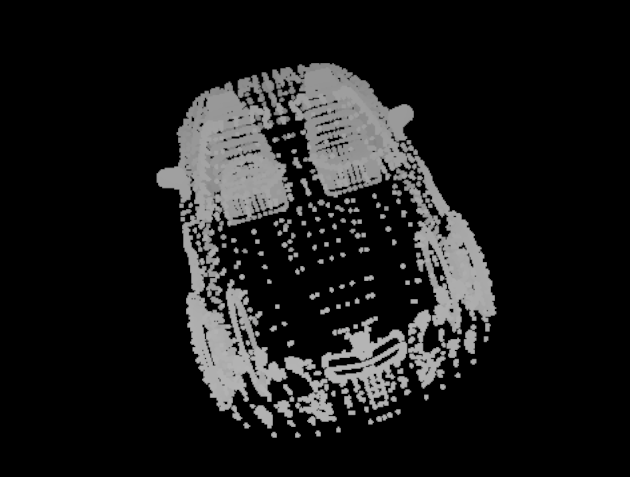
\includegraphics[height=35mm]{AudiA4_pointcloud}
    \hspace*{3mm}
    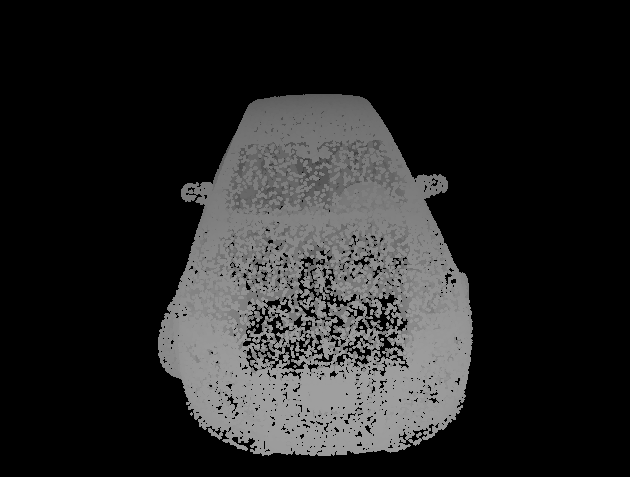
\includegraphics[height=35mm]{AudiA4_resampled}
    \caption{Audi A4 SketchUp Model before (left) and after (right) sampling.}
    \label{audia4resampled}
  \end{figure}

  
\section{Matching Scanned Objects with Generated 3D Point Clouds}

To find the desired object in the outdoor scene, the 3D laser scan is
segmented. We exploit the assumptions that all objects are on the
ground, i.e., a car always has the wheels on the ground and so do the
downloaded models. Therefore the first step is to remove the
ground. For this purpose, we use the approach described by Stiene et
al. in~\cite{Stiene:2006}. The points are converted into cylindrical
coordinates and the nearest neighbor within the vertical sweep plane
is identified. The angular gradient defines the nature of the point
(ground or not ground). Fig.~\ref{groundremoved} shows the obtained
result. The components of the scan become distinguishable and
spatially disconnected.
  
  \begin{figure}
\centering
      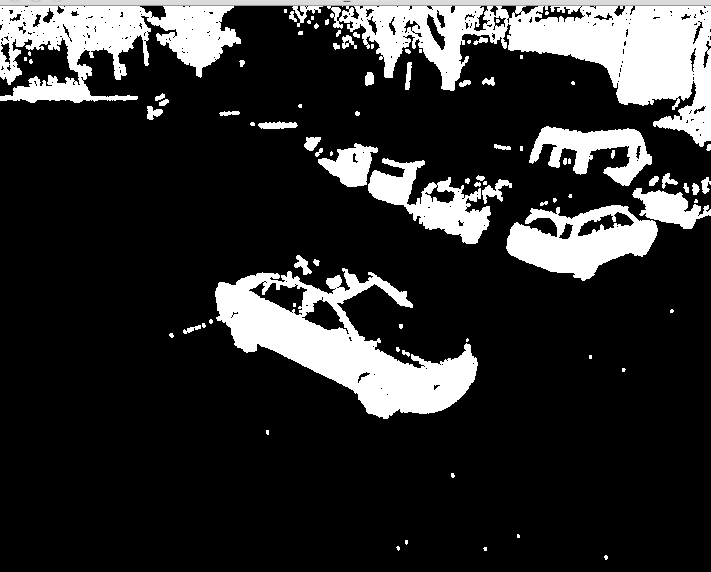
\includegraphics[height=50mm]{ground-removed}
    \caption{Scan with the ground points removed}
    \label{groundremoved}
  \end{figure}

After the ground has been removed, we automatically select an object
with an interactively provided starting guess. First, we find the
point $p$ which is closest to the starting guess. Then, a region is
grown around $p$ by iteratively adding points $p'$ satisfying the
conditions $p_x - \epsilon \leq p'_x \leq p_x + \epsilon$, $p_y -
\epsilon \leq p'_y \leq p_y + \epsilon$, $p_z - \epsilon \leq p'_z
\leq p_z + \epsilon$. To quickly find the points which match the
criteria a $k$-d tree is used. The $\epsilon$ threshold is dependent
on the point density of the scans and the distance from the scan
origin to the starting guess. Fig.~\ref{segmented_object} (left)
shows an obtained segmented object.
	
\begin{figure}[Ht]
  \centering
  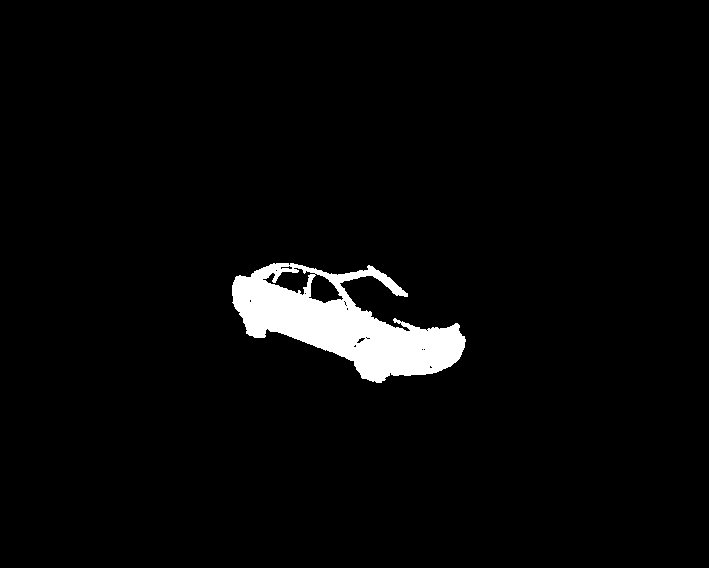
\includegraphics[height=30mm]{audi_segmented}
  \hfill
  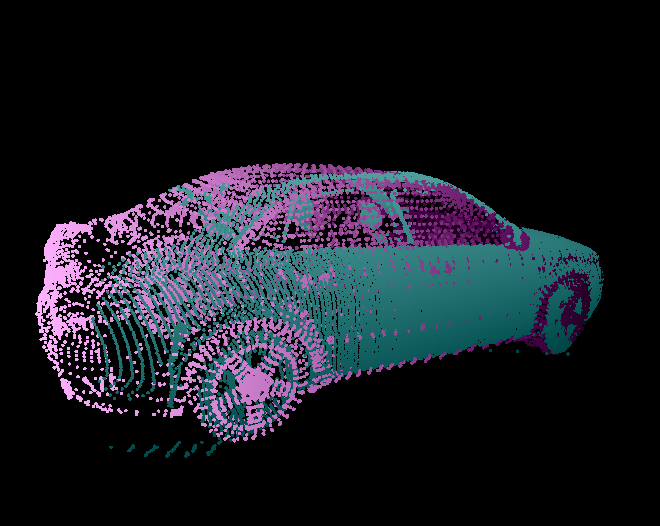
\includegraphics[height=30mm]{step4}
  \hfill
  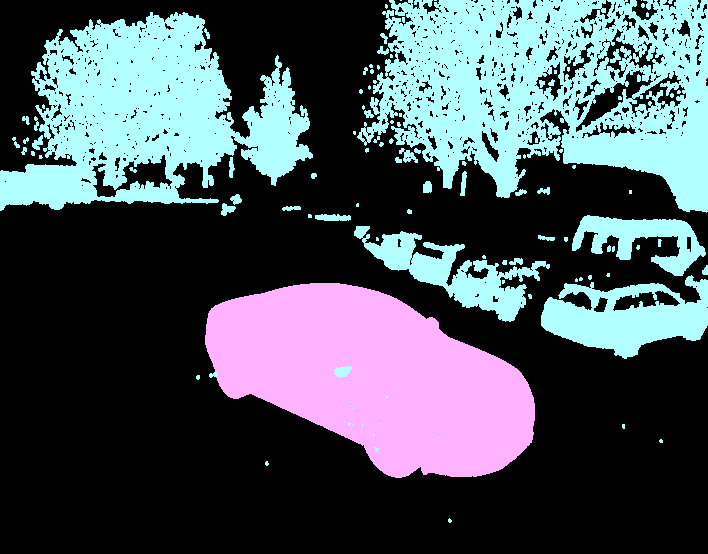
\includegraphics[height=30mm]{recovery_model_in_big_scan}
  \caption{Left: Segmented Audi A4. Middle: Audi A4 scan and model matched using SICP (magenta model and cyan scan data). Right: Recovered transformation matrix and application to positioning the object in the scan.}
  \label{segmented_object}
\end{figure}

A complete automatic system repeatedly applies the above scheme using
random points as starting guesses. Region growing is applied to
automatically segment the environment scan. The procedure is repeated
with the remaining points, thus obtaining non-overlapping
components. Regions with at least 500 points are considered valid
object candidates. They are centered in their respective centroid and
scaled in the $\alpha$-bounding box as in the interactive scheme.

Afterwards, the obtained segmented objects and the Google Warehouse
models are matched using a variant of iterative closest points
algorithm (SICP). ICP determines the translation and rotation between
the two point clouds (object and model), but it does not include the
scale factor. Following the derivation for the scale factor by
Horn~\cite{Horn:1987}, we compute for $n$ matching points of the two
point clouds (\emph{model} and \emph{scan}) $\{p_{m,i}\}$ and $\{p_{s,
  i}\}$ (both centered in their respective centroid):
%
\begin{align*}
  & s = \sqrt{\nicefrac{\sum\limits_{i=1}^n ||p_{m,i}||^2}{\sum\limits_{i=1}^n ||p_{s,i}||^2}}.
\end{align*}
% The advantage of the formula above is that rotation is not required
to determine the scale factor. However, it requires symmetric point
matching in ICP: points from both left and right are matched with
their closest counterpart. Initially, the maximum matching distance
between points, $\Delta$, is large to enforce coarse alignment. This
scales the model roughly to the same size as the segmented object. We
run \emph{i} iterations with this distance or until the error
converges. The matching is further refined by running the same number
of iterations with a smaller maximum distance, $\delta$. This step
allows fine matchings between points and the objects are consequently
perfectly aligned. Fig.~\ref{segmented_object} (middle) shows a
result of the matching between scan and model using SICP.  The right
subfigure shows the model aligned with its equivalent object in the
initial scan.

\iffalse
SICP returns a $4 \times 4$ matrix $M$, which represents the transformation between model and scan. The preprocessing step performed on both model and segmented object is stored in matrix $A$:

\begin{align*}
	& A = \begin{pmatrix}
		s & 0 & 0 & t_x \cdot s \\
		0 & s & 0 & t_y \cdot s \\
		0 & 0 & s & t_z \cdot s \\ 
		0 & 0 & 0 & 1 \\
		\end{pmatrix}
\end{align*}

where $s = \alpha / max$, $max$ is the maximum absolute coordinate after centering, and $t = (t_x, t_y, t_z)$ is the centering translation. The final transformation matrix needed for the correct alignment of the model in the initial scan is: $ T = M^{-1} \cdot A$. Fig.~\ref{segmented_object}(c) shows the model aligned with its equivalent object in the initial scan.
\fi

\section{Evaluation Metrics}

Running the matching algorithm and applying the recovery
transformations results in two sets of 3D points which share the same
coordinate system: $S$ -- the scan, and $M$ -- the model. It is
important to note that the scanned set depends on the scanner view
point and has occluded parts. We designed an error function which
penalizes points in the scan without model correspondence.

Let $c(p) \in M$ be the point in the model which is closest to $p$ by
Euclidean distance. Then, the error function is defined as:
%
\begin{align*}
	E &= \frac{\sum_{i=1}^{|M|} dist(M_i, c(M_i))}{|M|}
\end{align*}
%
A small $E$ denotes a very good match, while larger $E$ values suggest
either a poor model or a different object. In the experiments we
discovered that the error function also ranks models by similarity to
the original scanned object.

\section{Experiment and Results}

We acquired several scans using a Riegl VZ-400 3D laser scanner in the
Jacobs University Bremen parking lot, without focusing on any
particular car. Each scan has roughly 4 million 3D points and 5 cars
were segmented. For each segmented object we automatically downloaded
its corresponding models from Google Warehouse and ran SICP with 4
starting rotations as $(\theta_x,\theta_y,\theta_z)$, where $\theta_y$
specifies the rotation around the vertical axis. We only consider the
rotation around the $y$ axis and used four initial angles, i.e., $0,
\nicefrac{\pi}{2}, \pi$ and $\nicefrac{3\pi}{2}$. 

\begin{figure}
  \centering
  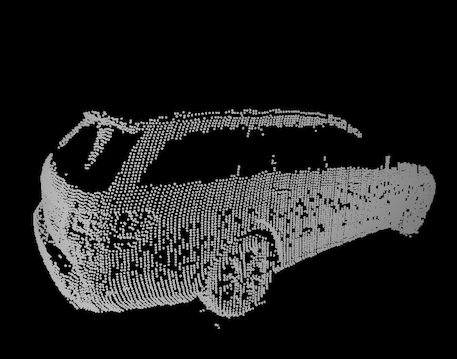
\includegraphics[height=25mm]{chapter5_pictures/Mercedes}
  \hfill
  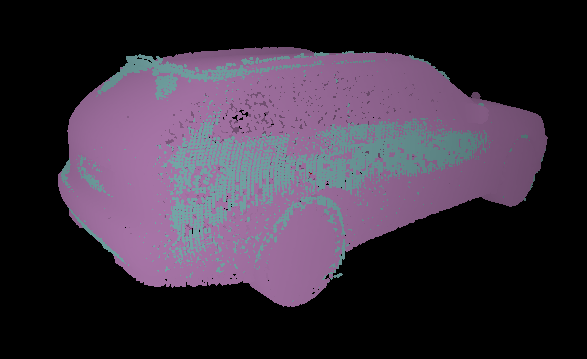
\includegraphics[height=25mm]{chapter5_pictures/Mercedes_matched}
  \hfill
  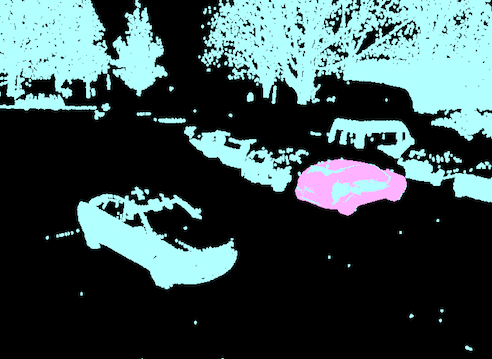
\includegraphics[height=25mm]{chapter5_pictures/Mercedes_matched_scan}
  \caption{Segmented Mercedes C350 and its best SICP match.}
  \label{mercedes_trio}
\end{figure}

The first segmented car, a Mercedes C350 (see
Fig.~\ref{mercedes_trio}), contains 8920 points and we downloaded all
89 models available in Google Warehouse. This car presented a large
number of very accurate models and the results are observed in
tables~\ref{mercedes_results_good} and~\ref{mercedes_results_bad}. In
each column, we present the error value on the left, the starting
rotation used to obtain this score and the image of the model provided
by Google Warehouse. The 89 models downloaded contain not only cars,
but also random components as chosen by their creators. Our error
function ranks the accurate car models first. As the models resemble
less a Mercedes C350, they have a lower rank and the very last are
other random objects, which do not resemble a car at all. The Mercedes
C350 is a good balance between the quality of the segmented object and
reliable collection of 3D models.

  \begin{longtable}{p{25mm}p{35mm}c}
  \caption{Mercedes C350 - Best matched models (3)}
  \label{mercedes_results_good}\\
  \multicolumn{1}{c}{\centering \textbf{Error}} & \multicolumn{1}{c}{\textbf{Y-axis Rotation}} & \multicolumn{1}{c}{\textbf{Google SketchUp model}} \\[1.2ex]
  \endfirsthead

  \multicolumn{3}{c}%
  {{\tablename\ \thetable{} -- continued from previous page}} \\
  \multicolumn{1}{c}{\textbf{Error}} &
  \multicolumn{1}{c}{\textbf{Y-axis Rotation}} &
  \multicolumn{1}{c}{\textbf{Google SketchUp model}} \\
  \endhead

  \multicolumn{3}{r}{{Continued on next page}} \\
  \endfoot

  \endlastfoot

  	\centering $49.0$ & \centering $\nicefrac{\pi}{2}$ & \begin{minipage}{40mm}{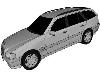
\includegraphics{models/1c5a350ea0f55f793fbce9ec40e1f047.jpg}}\end{minipage}\\
  	\centering $49.0$ & \centering $\nicefrac{\pi}{2}$ & \begin{minipage}{40mm}{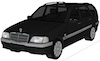
\includegraphics{models/689346b4812ead699bdae02f855f706c.jpg}}\end{minipage}\\
  	\centering $49.0$ & \centering $\nicefrac{\pi}{2}$ & \begin{minipage}{40mm}{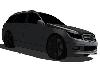
\includegraphics{models/875bc6efc7f33c052e877e82c90c24d.jpg}}\end{minipage}\\
  \end{longtable}

  \begin{longtable}{p{25mm}p{35mm}c}
  \caption[Mercedes C350]{Mercedes C350 - Models with high error (2)}\\
  \label{mercedes_results_bad}\\

  \multicolumn{1}{c}{\centering \textbf{Error}} & \multicolumn{1}{c}{\textbf{Y-axis Rotation}} & \multicolumn{1}{c}{\textbf{Google SketchUp model}} \\[1.2ex]
  \endfirsthead

  \multicolumn{3}{c}%
  {{\tablename\ \thetable{} -- continued from previous page}} \\
  \multicolumn{1}{c}{\textbf{Error}} &
  \multicolumn{1}{c}{\textbf{Y-axis Rotation}} &
  \multicolumn{1}{c}{\textbf{Google SketchUp model}} \\
  \endhead

  \multicolumn{3}{r}{{Continued on next page}} \\
  \endfoot

  \endlastfoot
  	\centering $19865.0$ & \centering $\nicefrac{3\pi}{2}$ & \begin{minipage}{40mm}{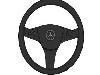
\includegraphics{models/c023011d5ada6bd9b1bb46d2556ba67d.jpg}}\end{minipage}\\
  	\centering $21221.0$ & \centering $0$ & \begin{minipage}{40mm}{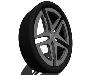
\includegraphics{models/951b1572b316980de341b5704aa568bd.jpg}}\end{minipage}\\
  \end{longtable}

  \begin{figure}
    \centering
    \subfloat[Segmented Audi A4]{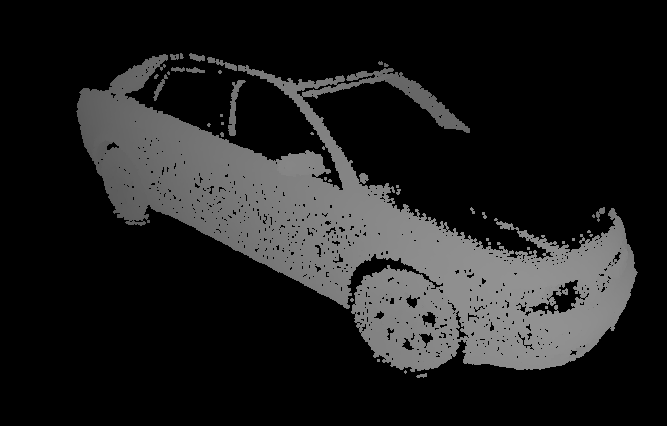
\includegraphics[height=23mm]{chapter5_pictures/Audi}}
    \hfill
    \subfloat[Best match]{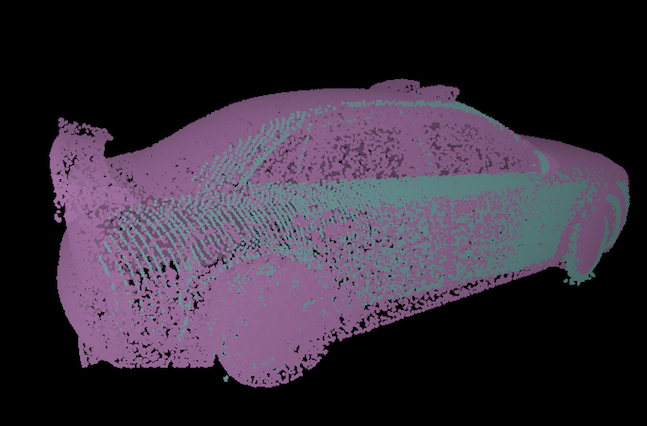
\includegraphics[height=23mm]{chapter5_pictures/Audi_matched}}
    \hfill
    \subfloat[Scan with matched Audi A4]{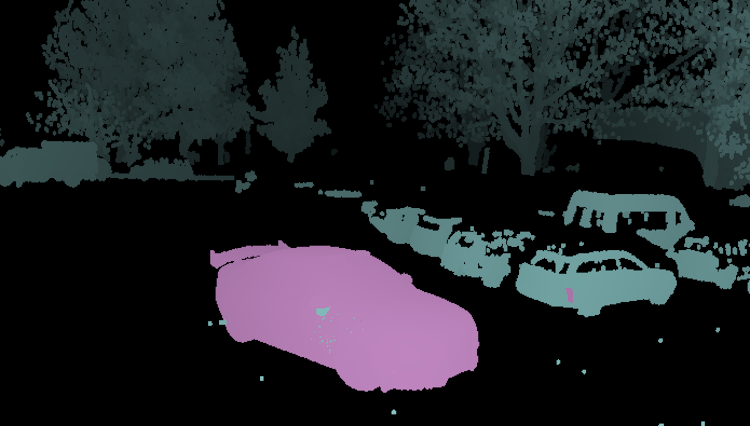
\includegraphics[height=23mm]{chapter5_pictures/Audi_matched_scan}}
    \caption{Segmented Audi A4 and its best SICP match.}
    \label{audi_trio}
  \end{figure}

We extracted an Audi A4 from the environment scan containing 18801
points and we found 80 models responding to the equivalent search
query. Unlike the Mercedes, the models vary more and have additional
decorations. The error function does not take into consideration the
model's unmatched points, because in every case the model contains
more points than the segmented object. In contrast, the segmented
object has points on maximum 3 sides. To solve this problem, a shape
descriptor could be used to differentiate between models with extra
elements. Being a sports car, Audi A4 is prone to user design
experiments, thus making the model collection less reliable in some
respects (Fig.~\ref{audi_trio}).

  \begin{figure}
    \centering
    \subfloat[Segmented Volkswagen Golf]{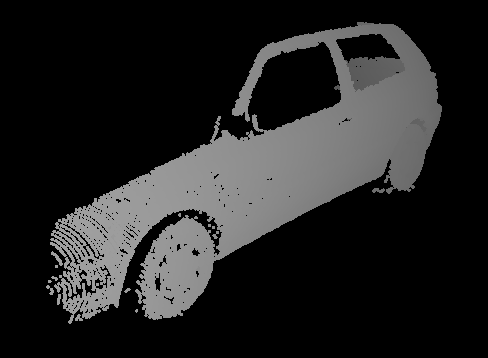
\includegraphics[height=25mm]{chapter5_pictures/Golf}}
    \hspace{3 mm}
    \subfloat[Best match]{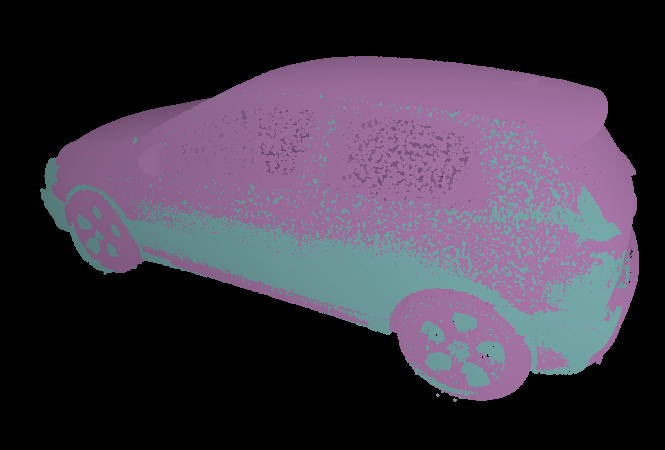
\includegraphics[height=25mm]{chapter5_pictures/Golf_matched}}
    \hspace{3 mm}
    \subfloat[Scan with matched Volkswagen Golf]{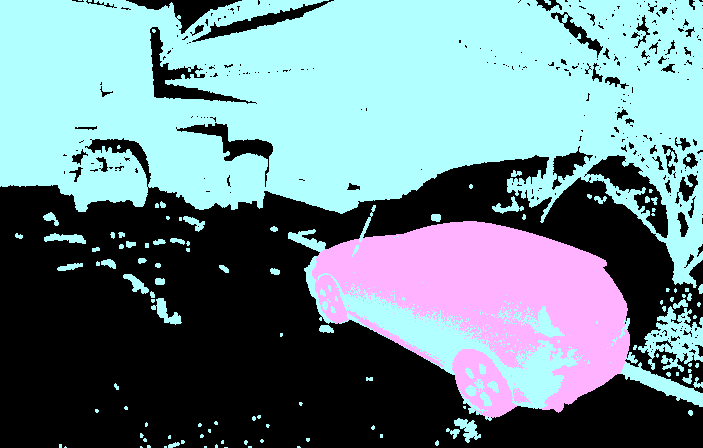
\includegraphics[height=25mm]{chapter5_pictures/Golf_matched_scan}}
    \caption{Segmented Volkswagen Golf and its best SICP match.}
    \label{golf_trio}
  \end{figure}

The extracted Volkswagen Golf is an unidentified older version of the
popular German car and it has 44686 points and 233 downloaded
models. The difficulties in matching this model stem out exactly from
the fact that it is an old version and the models in Google Warehouse
focus mostly on the latest Golf models. However, SICP identified and
ranked higher the models resembling an older version as opposed to
newer versions of the same car (Fig.~\ref{golf_trio}).
 
  \begin{figure}
    \centering
    \subfloat[Segmented Renault Kangoo]{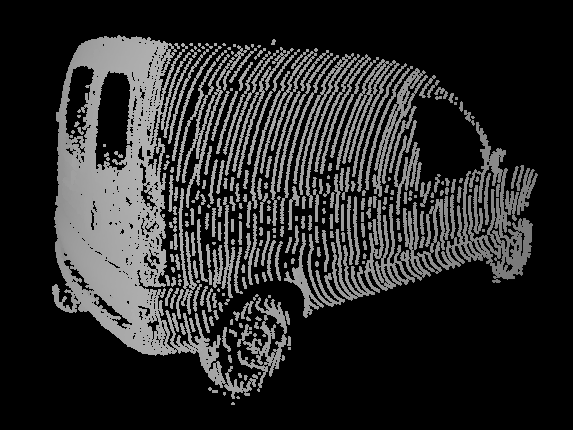
\includegraphics[height=29mm]{chapter5_pictures/Renault}}
    \hspace{3 mm}
    \subfloat[Best match]{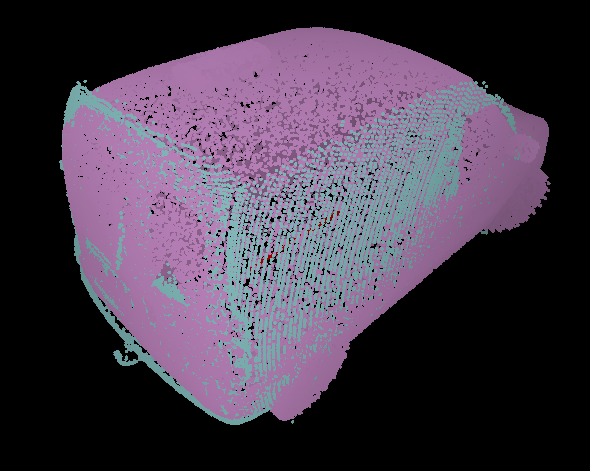
\includegraphics[height=29mm]{chapter5_pictures/Renault_matched}}
    \hspace{3 mm}
    \subfloat[Scan with matched Renault Kangoo]{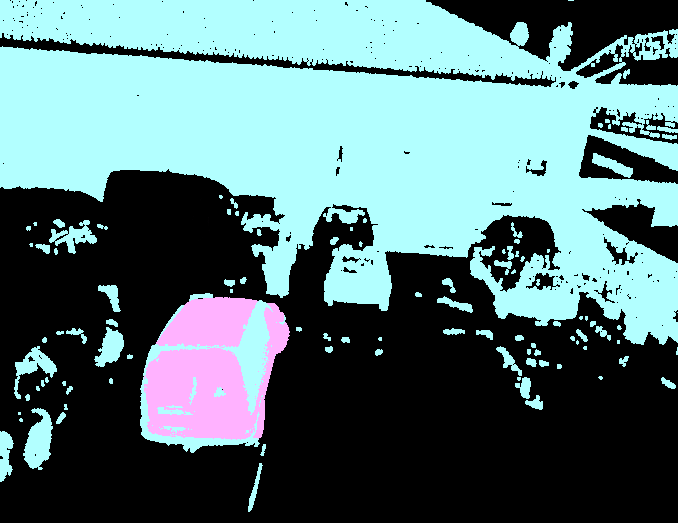
\includegraphics[height=29mm]{chapter5_pictures/Renault_matched_scan}}
    \caption{Segmented Renault Kangoo and its best SICP match.}
    \label{renault_trio}
  \end{figure}

Another class of cars is represented by a segmented Renault Kangoo,
containing 13597 points and with 18 models in Google Warehouse. Even
though the number of available models is reduced, they have a very
good quality and we found a very good match. This suggests that the
proposed algorithm is not only fit for small cars or limousines, but
also for larger objects such as vans (Fig.~\ref{renault_trio}).

  \begin{figure}[Ht]
    \centering
    \subfloat[Segmented Citroen C5]{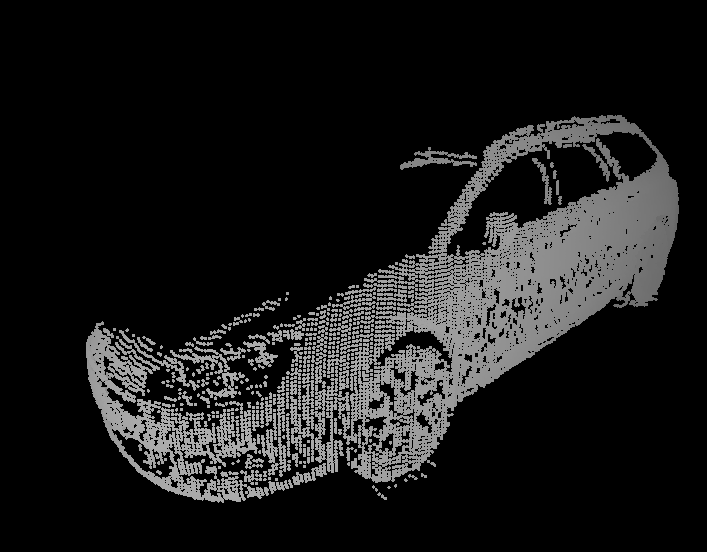
\includegraphics[height=25mm]{chapter5_pictures/Citroen}}
    \hspace{3 mm}
    \subfloat[Best match]{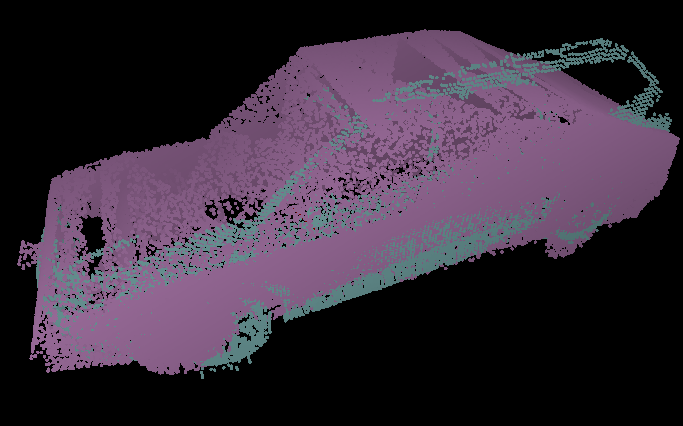
\includegraphics[height=25mm]{chapter5_pictures/Citroen_matched}}
    \hspace{3 mm}
    \subfloat[Scan with matched Citroen C5]{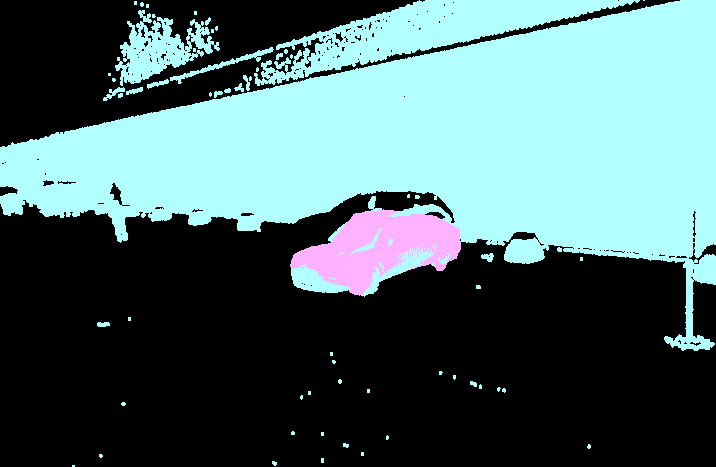
\includegraphics[height=25mm]{chapter5_pictures/Citroen_matched_scan}}
    \caption{Segmented Citroen C5 and its best SICP match.}
    \label{citroen_trio}
  \end{figure}

The last segmented vehicle is a Citroen C5 with 10089 points and only
11 available models in Google Warehouse. Unlike the previous car, the
quality of these models is very low and all SICP matchings have a high
error rate as it can be observed in Fig.~\ref{citroen_trio}. This
means that for the less popular type of cars Google Warehouse is
useful in identifying the class of the object, but it is probably not
enough in determining a finer classification and finding out the brand
of the car.

We considered the segmented Mercedes C350 versus the top 3 models from
all the other cars. SICP ranked the models starting with the Mercedes
C350 as being the best, followed by two Audis, then, with larger
errors, Citroen and lastly Golf and Renault. SICP found the right
brand of car among different models and moreover, the next matched
models were similar in shape and size with the segmented car, which
gives us an insight in similar shapes and objects that share
particular properties as observed in table \ref{mercedes_vs_all}.

  \begin{longtable}{p{25mm}p{35mm}c}
  \caption[Mercedes C350]{Mercedes C350 vs different car brand models (10)}\\
  \label{mercedes_vs_all}\\

  \multicolumn{1}{c}{\centering \textbf{Error}} & \multicolumn{1}{c}{\textbf{Y-axis Rotation}} & \multicolumn{1}{c}{\textbf{Google SketchUp model}} \\[1.2ex]
  \endfirsthead

  \multicolumn{3}{c}%
  {{\tablename\ \thetable{} -- continued from previous page}} \\
  \multicolumn{1}{c}{\textbf{Error}} &
  \multicolumn{1}{c}{\textbf{Y-axis Rotation}} &
  \multicolumn{1}{c}{\textbf{Google SketchUp model}} \\
  \endhead

  \multicolumn{3}{r}{{Continued on next page}} \\
  \endfoot

  \endlastfoot

  	\centering $49.0$ & \centering $\nicefrac{\pi}{2}$ & \begin{minipage}{40mm}{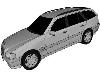
\includegraphics{models/1c5a350ea0f55f793fbce9ec40e1f047.jpg}}\end{minipage}\\
  	\centering $49.0$ & \centering $\nicefrac{\pi}{2}$ & \begin{minipage}{40mm}{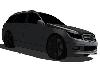
\includegraphics{models/875bc6efc7f33c052e877e82c90c24d.jpg}}\end{minipage}\\
  	\centering $57.0$ & \centering $\nicefrac{\pi}{2}$ & \begin{minipage}{40mm}{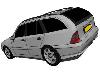
\includegraphics{models/eb5a5eb751cca94a3fbce9ec40e1f047.jpg}}\end{minipage}\\
  	\centering $59.0$ & \centering $0$ & \begin{minipage}{40mm}{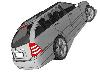
\includegraphics{models/a0c60115f83f1f77b1bb46d2556ba67d.jpg}}\end{minipage}\\
  	\centering $60.0$ & \centering $0$ & \begin{minipage}{40mm}{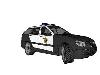
\includegraphics{models/5bab0881b7a18b12733269057ed164db.jpg}}\end{minipage}\\
  \end{longtable}

We matched an Audi A4 with all objects automatically segmented by
using the best matched Audi A4 as the model. By applying the growing
regions algorithm we identified $67$ candidate objects and the best matches are shown in Table~\ref{audi_big_scan}.

\begin{longtable}{p{25mm}p{35mm}c}
\caption[Find Audi A4 in entire scan]{Find Audi A4 in entire scan}\\
\label{audi_big_scan}\\

\multicolumn{1}{c}{\centering \textbf{Error}} & \multicolumn{1}{c}{\textbf{Y-axis Rotation}} & \multicolumn{1}{c}{\textbf{Object}} \\[1.2ex]
\endfirsthead

\multicolumn{3}{c}%
{{\tablename\ \thetable{} -- continued from previous page}} \\
\multicolumn{1}{c}{\textbf{Error}} &
\multicolumn{1}{c}{\textbf{Y-axis Rotation}} &
\multicolumn{1}{c}{\textbf{Object}} \\
\endhead

\multicolumn{3}{r}{{Continued on next page}} \\
\endfoot

\endlastfoot

	\centering $105.0$ & \centering $\nicefrac{\pi}{2}$ & \begin{minipage}{40mm}{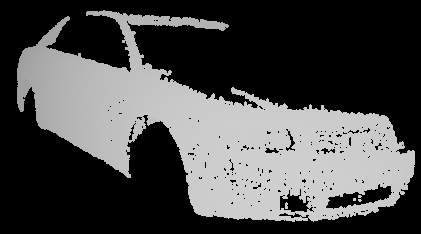
\includegraphics[width=50mm]{objects/audi}}\end{minipage}\\
	\centering $178.0$ & \centering $\nicefrac{\pi}{2}$ & \begin{minipage}{40mm}{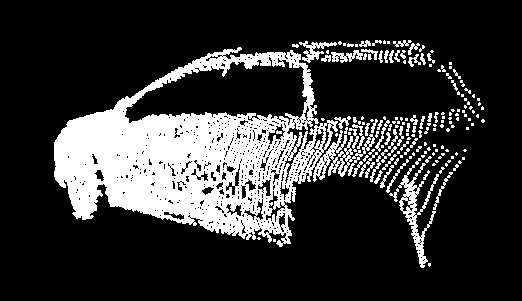
\includegraphics[width=50mm]{objects/other_car}}\end{minipage}\\
	\centering $400.0$ & \centering $\nicefrac{\pi}{2}$ & \begin{minipage}{40mm}{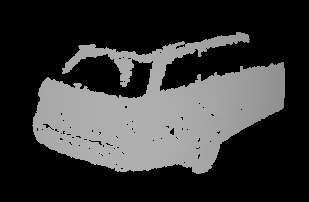
\includegraphics[width=50mm]{objects/other_car_2}}\end{minipage}\\
\end{longtable}

The best matching object is the Audi A4. The next two best-matching
objects are also cars, but different brands. The rest of the objects
have error values of $2000$ to $77000$ and are thus very poor matches.

\section{Conclusion and Future Work}

In conclusion, the current work presents a feasible approach, proven
to work in practice by thorough experiments and results, which solves
the problem of identifying a given object in an outdoor
environment. Semantic mapping is thus improved and the method is
applicable for a better understanding of the scene. The work raises a
myriad of new questions and future work sheds some light on short term
and long term improvements for SICP.

The error function presented does not take in account extra points
which are present on the model but not on the scan. A further
difficulty in the attempt to improve the error function is that the
glass areas of cars are not captured by a laser scanner. In future
work, we plan to project all points to a plane and compare the
resulting 2-dimensional convex hull shapes by shared surface.

Our current work focuses on outdoor scans in urban environments and
does not cover any experiments with indoor data. One very important
assumption for our rotation model is that the objects are on the
ground, thus favoring rotations on the y-axis. While the major indoor
objects (chairs, tables etc.) are similar in nature to the outdoor
objects, refining to smaller, harder segmentable objects with unknown
rotations (objects on a shelf) is an open problem. Solving this issue
is important in the context of completely identifying real-world
objects with Google SketchUp models.

The candidate models are currently found based on the search results
of Google Warehouse database. However, it is desired to identify a
scanned object with a SketchUp model without a search string. For this
purpose, further research work is needed in order to devise an
accurate classifier. We currently have no methods to reject objects
which share no similarities to the real-world scanned object without
running the SICP algorithm.

The presented method is extendable to a full-scene understanding
algorithm -- both labeling and completion of occluded areas. The SICP
algorithm is run on each real-world object of a segmented scan thus
finding the best matching SketchUp model and its orientation. The
real-world objects are then replaced with the SketchUp point cloud
thus resulting both a higher-resolution scan and semantic
labeling. Further work will be conducted to allow SICP to adjust
the guess based on future scans (backward corrections).

\bibliographystyle{plain}

\bibliography{lit,andreas_publication}

\end{document}
